\documentclass[a4paper, 11pt]{article}

% -- Coments
\usepackage{verbatim}

% ----- Fonts -----
% -- Fuente --
% \usepackage{fontspec}
% \setmonofont{JetBrainsMono Nerd Font}  

% -- Color --
\usepackage{xcolor}
%\definecolor{azul}{RGB}{00,33,99}
\definecolor{azul}{RGB}{35,72,180}

% -- Page Margin --
\usepackage[margin=1in]{geometry}

% -- Espaciados --
\newcommand{\Pspace}{0.5cm}
\newcommand{\Aspace}{0.2cm}

% -- Columnas --
\usepackage{multicol}

% -- Imagenes --
\usepackage{graphicx}
\usepackage{float}

% -- Matemáticas --
\usepackage{amsmath, amssymb}

% -- Gráficas --
\usepackage{pgfplots}
\pgfplotsset{compat=1.18}

% -- Código --
\usepackage{listings}
\lstset{
    language=Python,                   % Lenguaje del código
    basicstyle=\ttfamily\small,     % Fuente del código
    keywordstyle=\color{blue},      % Color de palabras clave
    commentstyle=\color{gray},      % Color de comentarios
    stringstyle=\color{red},        % Color de cadenas
    numbers=left,                   % Números de línea a la izquierda
    numberstyle=\tiny\color{gray},
    breaklines=true,                % Permitir saltos de línea
    frame=single                    % Marco alrededor del código
}

\begin{comment}
-- Formato de pregunta simple
    % - Problema n
    \vspace{\Pspace}
    \item Problema \par
        % Respuesta:
        \vspace{\Aspace} \par
        { \color{azul}  }


 -- Formato de pregunta multimple
        % - Problema 
        \vspace{\Pspace}
        \item  \par
             % Respuestas:
            \vspace{\Aspace} \par
            a) 
            \\ { \color{azul} }

            \vspace{\Aspace} \par
            b) 
            \\ { \color{azul} }


 -- Formato de imagen
\begin{figure}[!ht]
    \centering
    \includegraphics[width=0.5\textwidth]{}
\end{figure}


 -- Formato de tabla
\begin{tabular}{c|c}
    \textbf{A} & \textbf{B} \\
    \hline
    Texto & Texto \\
    Texto & Texto
\end{tabular} \\
\end{comment}


\title
{
    Análisis de algoritmos 2026-1 \\
    Tarea 1
}

    \begin{document}

    \maketitle

    \begin{center}
        \begin{tabular}{r|l}
            \textbf{Expediente} & \textbf{Nombre} \\ \hline
            219208106 & Bórquez Guerrero Angel Fernando \\
        \end{tabular}
    \end{center}

    \rule{\linewidth}{0.3mm}

    \vspace{0.3cm}
    \section{Condiciones iniciales}
    En este proyecto se analiza el comportamiento de tres algoritmos clásicos de ordenamiento: Insertion Sort, Selection Sort y Merge Sort. El objetivo es comparar su desempeño al ordenar arreglos bajo distintas condiciones de entrada. \par

    Para realizar el experimento se generaron arreglos de diferentes tamaños, los cuales serán utilizados como entrada para cada uno de los algoritmos. Los tamaños considerados en este estudio son los siguientes: \\
\begin{lstlisting}
sizes = [1000, 5000, 10000, 15000, 20000, 25000, 30000, 
         35000, 40000, 45000]
\end{lstlisting}

Para cada tamaño se generan 30 arreglos en total, distribuidos en tres tipos de orden inicial:
\begin{enumerate}
    \item \textbf{10 arreglos crecientes}, donde los elementos ya se encuentran ordenados.
    \item \textbf{10 arreglos decrecientes}, representando el caso inverso al ordenado.
    \item \textbf{10 arreglos aleatorios}, donde los elementos aparecen en posiciones sin ningún orden particular.
\end{enumerate}
De esta manera es posible observar cómo cambia el rendimiento de cada algoritmo dependiendo de la estructura inicial de los datos. \par

La generación de los arreglos se realiza utilizando la librería NumPy, la cual permite crear conjuntos de números aleatorios de manera eficiente. Además, se utiliza un random seed para garantizar la reproducibilidad del experimento. Esto significa que cada vez que el código se ejecute con el mismo valor de semilla se generarán exactamente los mismos arreglos, permitiendo repetir las pruebas y obtener resultados consistentes.

\newpage
\subsection{Implementación}
El código utilizado para generar los arreglos es el siguiente:
\begin{lstlisting}
import numpy as np

def create_array(size, order, seed=42):
np.random.seed(seed)

arreglo = np.random.randint(0, 10000, size=size)
    
if order == 'creciente':
    return np.sort(arreglo)
elif order == 'decreciente':
    return np.sort(arreglo)[::-1]
elif order == 'aleatorio':
    return arreglo
\end{lstlisting}
Esta función permite generar arreglos de un tamaño determinado y con el tipo de orden inicial requerido para las pruebas, lo que facilita la automatización del proceso de experimentación.



\section{Insertion-Sort}
Una propiedad interesante de este algoritmo es que su rendimiento depende fuertemente del orden inicial del arreglo. Cuando los datos ya están ordenados, el algoritmo realiza muy pocos movimientos. En cambio, cuando los datos están en orden inverso, debe desplazar casi todos los elementos en cada iteración, lo que incrementa considerablemente el tiempo de ejecución.

\subsection{Implementación}
El código utilizado para implementar Insertion Sort es el siguiente:
\begin{lstlisting}
def insertion_sort(arr):
    for n in range(1, len(arr)):
        key = arr[n]
        i = n - 1

        while(i >= 0 and key < arr[i]):
            arr[i + 1] = arr[i]
            i -= 1
        arr[i + 1] = key

    return arr
\end{lstlisting}


\newpage
\subsection{Resultados}
La tabla muestra los tiempos de ejecución obtenidos para los diferentes tamaños de arreglo y tipos de orden inicial.

\begin{table}[H]
\centering
\begin{tabular}{|l|c|r|}
\hline
Orden & Tamaño & Tiempo (s) \\
\hline
creciente & 1000 & 0.000067 \\
creciente & 5000 & 0.000350 \\
creciente & 10000 & 0.000852 \\
creciente & 15000 & 0.000831 \\
creciente & 20000 & 0.001127 \\
creciente & 25000 & 0.001388 \\
creciente & 30000 & 0.001784 \\
creciente & 35000 & 0.001900 \\
creciente & 40000 & 0.002355 \\
creciente & 45000 & 0.002483 \\
\hline
decreciente & 1000 & 0.021736 \\
decreciente & 5000 & 0.622290 \\
decreciente & 10000 & 2.508498 \\
decreciente & 15000 & 5.708101 \\
decreciente & 20000 & 10.258179 \\
decreciente & 25000 & 15.993664 \\
decreciente & 30000 & 23.019070 \\
decreciente & 35000 & 31.383729 \\
decreciente & 40000 & 41.403777 \\
decreciente & 45000 & 52.451626 \\
\hline
aleatorio & 1000 & 0.012250 \\
aleatorio & 5000 & 0.329701 \\
aleatorio & 10000 & 1.309284 \\
aleatorio & 15000 & 2.886151 \\
aleatorio & 20000 & 5.253931 \\
aleatorio & 25000 & 8.254386 \\
aleatorio & 30000 & 11.958789 \\
aleatorio & 35000 & 16.309728 \\
aleatorio & 40000 & 21.979351 \\
aleatorio & 45000 & 27.254113 \\
\hline
\end{tabular}
\caption{Tiempos de ejecución de Insertion Sort}
\end{table}


\newpage
\subsection{Gráfica de resultados}
La figura muestra la relación entre el tamaño del arreglo y el tiempo de ejecución del algoritmo para los diferentes tipos de orden inicial.

\begin{figure}[H]
\centering
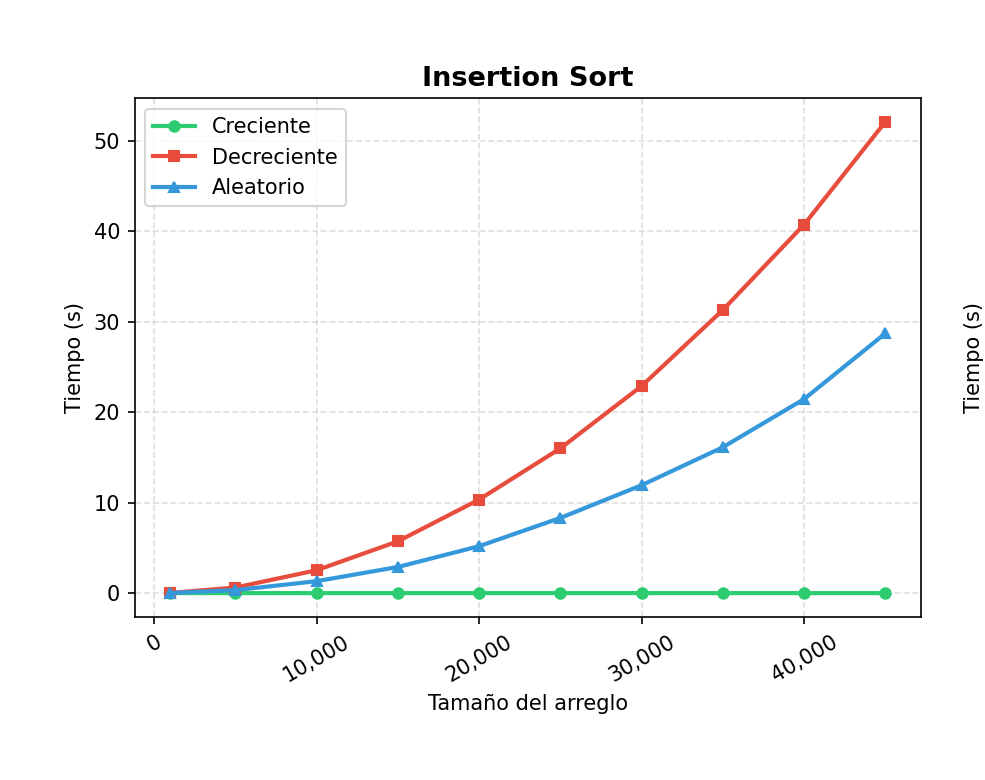
\includegraphics[width=0.6\textwidth]{graficas/insertion_sort.png}
\caption{Tiempo de ejecución de Insertion Sort}
\label{fig:insertion_graph}
\end{figure}


\subsection{Ajuste de funciones}
\subsubsection{Mejor caso (arreglo creciente)}
En el caso donde los datos se encuentran ordenados de forma creciente, Insertion Sort requiere muy pocos desplazamientos, ya que cada elemento se encuentra cerca de su posición final. Por esta razón, el tiempo de ejecución esperado teóricamente es del orden $O(n)$.
La figura muestra el ajuste de los datos experimentales a los modelos lineal y cuadrático.

\begin{figure}[H]
\centering
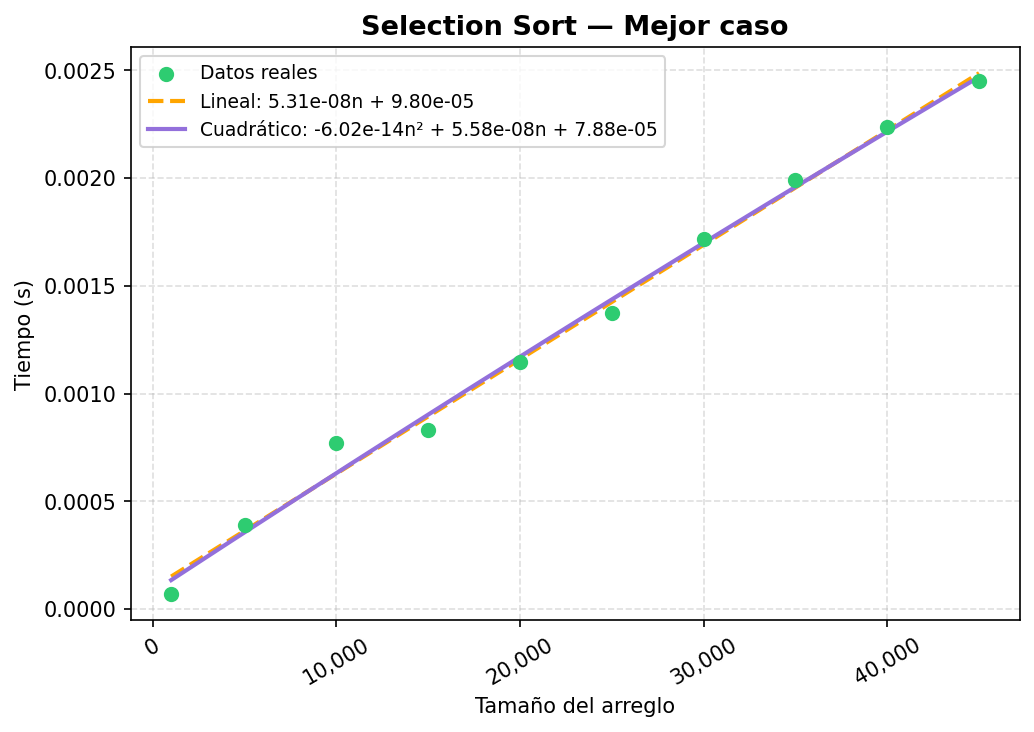
\includegraphics[width=0.6\textwidth]{graficas/insertion_sort_creciente.png}
\caption{Ajuste de funciones para el mejor caso de Insertion Sort}
\label{fig:insertion_best_fit}
\end{figure}

\newpage
\subsubsection{Peor caso (arreglo decreciente)}
Cuando el arreglo se encuentra en orden decreciente, cada nuevo elemento debe desplazarse hasta el inicio del arreglo para colocarse en su posición correcta. Esto produce el mayor número posible de comparaciones y desplazamientos dentro del algoritmo.
En este escenario, el comportamiento teórico esperado es cuadrático, es decir $O(n^2)$.

La Figura \ref{fig:insertion_worst_fit} muestra el ajuste de los datos experimentales utilizando los modelos lineal y cuadrático.
\begin{figure}[H]
\centering
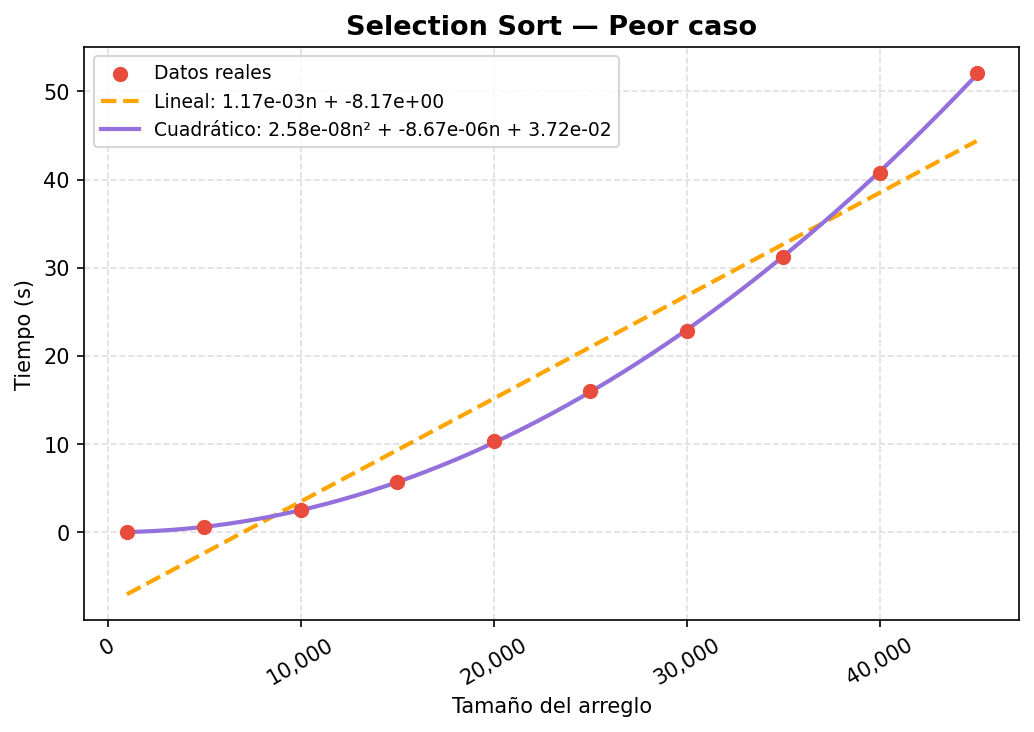
\includegraphics[width=0.6\textwidth]{graficas/insertion_sort_decreciente.png}
\caption{Ajuste de funciones para el peor caso de Insertion Sort}
\label{fig:insertion_worst_fit}
\end{figure}

\subsubsection{Caso promedio (arreglo aleatorio)}
En el caso promedio, donde los datos se encuentran en un orden aleatorio, el algoritmo debe realizar una cantidad significativa de desplazamientos para insertar cada elemento en su posición correcta.
El comportamiento esperado en este caso también es cuadrático, es decir $O(n^2)$, aunque con un crecimiento menor que en el peor caso.

La Figura \ref{fig:insertion_average_fit} muestra el ajuste de los datos experimentales a los modelos lineal y cuadrático.
\begin{figure}[H]
\centering
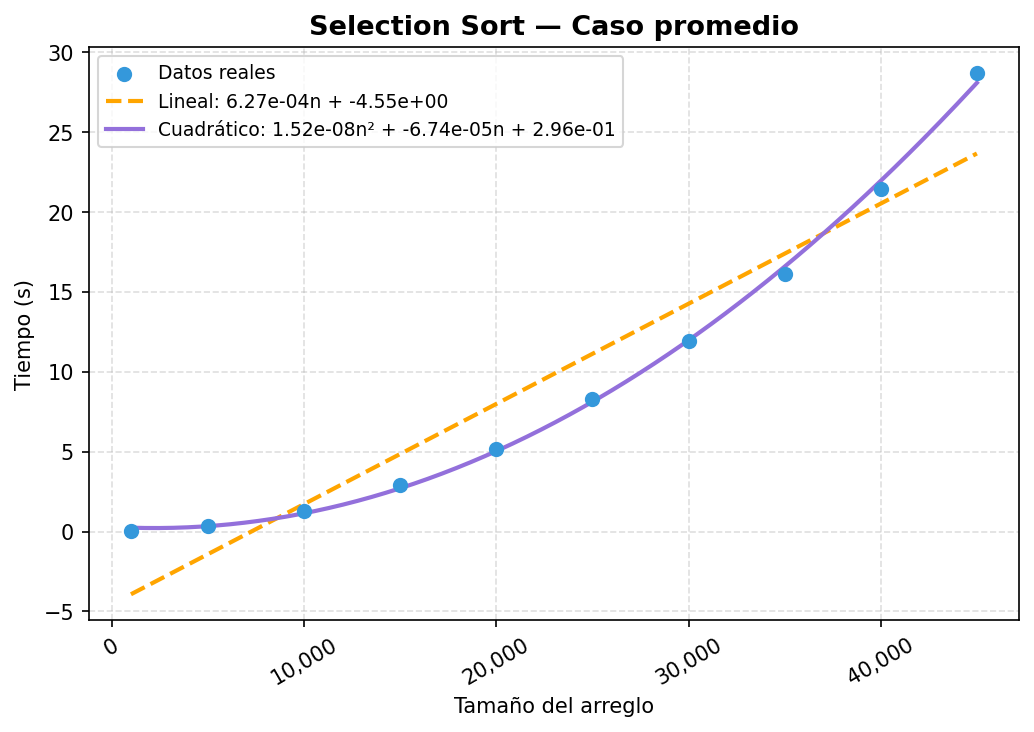
\includegraphics[width=0.6\textwidth]{graficas/insertion_sort_aleatorio.png}
\caption{Ajuste de funciones para el caso promedio de Insertion Sort}
\label{fig:insertion_average_fit}
\end{figure}





\newpage
\section{Selection Sort}
A diferencia de otros algoritmos como Insertion Sort, el número de comparaciones realizadas por Selection Sort es prácticamente el mismo independientemente del orden inicial de los datos. Por esta razón su tiempo de ejecución suele ser muy similar tanto para arreglos ordenados como para arreglos desordenados.

\subsection{Implementación}
El código utilizado para implementar Selection Sort en Python es el siguiente:

\begin{lstlisting}
def selection_sort(arr):
    n = len(arr)
    
    for i in range(n):
        min = i
        
        for j in range(i + 1, n):
            if arr[j] < arr[min]:
                min = j
        
        arr[i], arr[min] = arr[min], arr[i]
        
    return arr
\end{lstlisting}


\newpage
\subsection{Resultados}
La tabla muestra los tiempos de ejecución obtenidos para los diferentes tamaños de arreglo y tipos de orden inicial.

\begin{table}[H]
\centering
\begin{tabular}{|l|c|r|}
\hline
Orden & Tamaño & Tiempo (s) \\
\hline
creciente & 1000 & 0.012751 \\
creciente & 5000 & 0.316120 \\
creciente & 10000 & 1.030409 \\
creciente & 15000 & 2.340467 \\
creciente & 20000 & 3.940330 \\
creciente & 25000 & 6.455171 \\
creciente & 30000 & 8.925973 \\
creciente & 35000 & 12.387158 \\
creciente & 40000 & 15.924877 \\
creciente & 45000 & 20.572913 \\
\hline
decreciente & 1000 & 0.010388 \\
decreciente & 5000 & 0.270938 \\
decreciente & 10000 & 1.109008 \\
decreciente & 15000 & 2.498583 \\
decreciente & 20000 & 4.302078 \\
decreciente & 25000 & 6.814569 \\
decreciente & 30000 & 9.602518 \\
decreciente & 35000 & 13.023721 \\
decreciente & 40000 & 17.075167 \\
decreciente & 45000 & 21.685720 \\
\hline
aleatorio & 1000 & 0.009890 \\
aleatorio & 5000 & 0.252086 \\
aleatorio & 10000 & 1.038798 \\
aleatorio & 15000 & 2.320582 \\
aleatorio & 20000 & 4.245675 \\
aleatorio & 25000 & 6.438540 \\
aleatorio & 30000 & 9.517108 \\
aleatorio & 35000 & 13.197851 \\
aleatorio & 40000 & 17.312391 \\
aleatorio & 45000 & 22.033304 \\
\hline
\end{tabular}
\caption{Tiempos de ejecución de Selection Sort}
\label{tab:selection_results}
\end{table}


\newpage
\subsection{Gráfica de resultados}
La figura muestra la relación entre el tamaño del arreglo y el tiempo de ejecución del algoritmo para los diferentes tipos de orden inicial.

\begin{figure}[H]
\centering
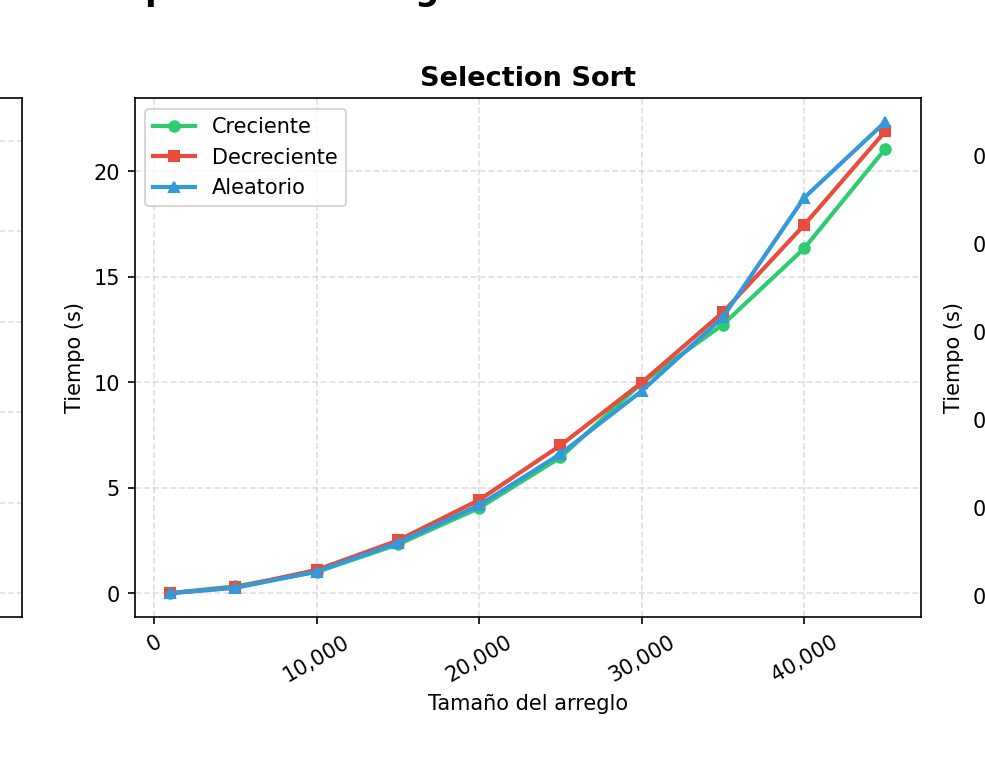
\includegraphics[width=0.6\textwidth]{graficas/selection_sort.png}
\caption{Tiempo de ejecución de Selection Sort}
\label{fig:selection_graph}
\end{figure}


\section{Ajuste de funciones}
\subsection{Arreglo creciente}

La Figura \ref{fig:selection_best_fit} muestra el ajuste de los datos experimentales para el caso en el que el arreglo se encuentra ordenado de forma creciente.

\begin{figure}[H]
\centering
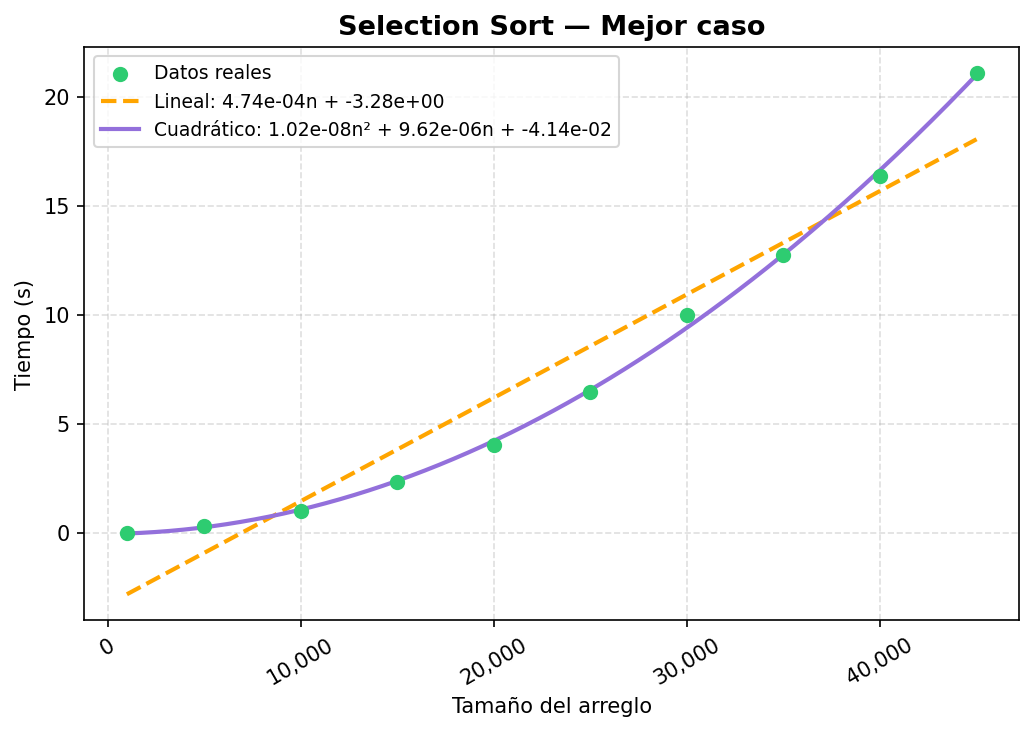
\includegraphics[width=0.6\textwidth]{graficas/selection_sort_creciente.png}
\caption{Ajuste por mínimos cuadrados para Selection Sort con arreglo creciente}
\label{fig:selection_best_fit}
\end{figure}

\newpage
\subsection{Arreglo decreciente}

La Figura \ref{fig:selection_worst_fit} muestra el ajuste de los tiempos de ejecución cuando el arreglo se encuentra en orden decreciente.

\begin{figure}[H]
\centering
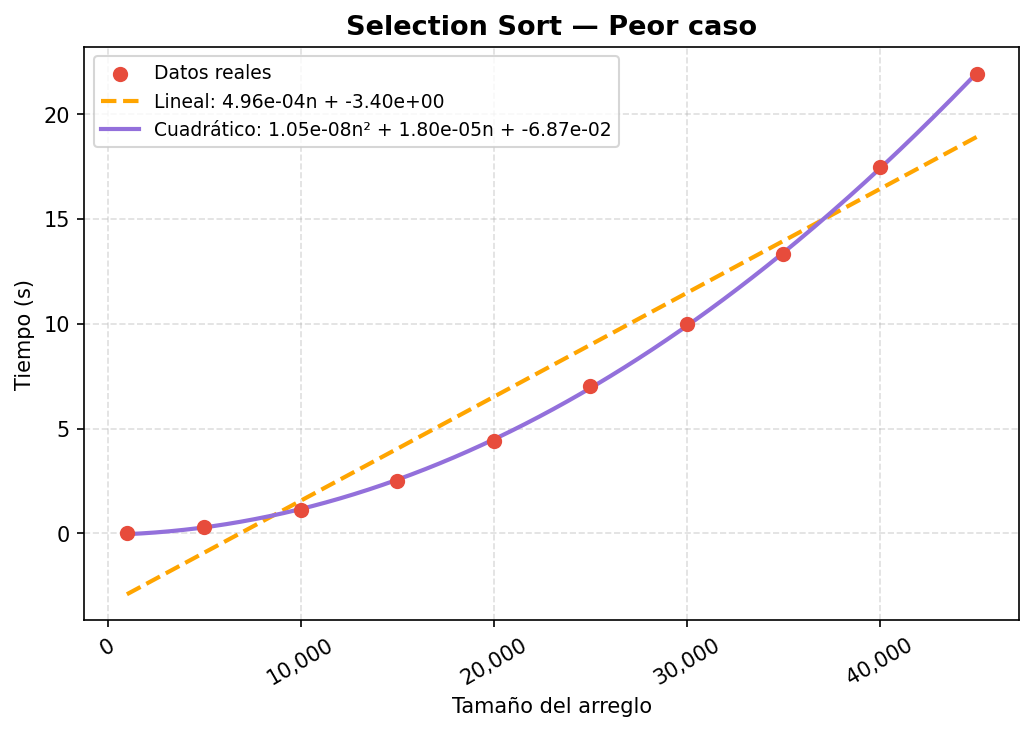
\includegraphics[width=0.6\textwidth]{graficas/selection_sort_decreciente.png}
\caption{Ajuste por mínimos cuadrados para Selection Sort con arreglo decreciente}
\label{fig:selection_worst_fit}
\end{figure}

\subsection{Arreglo aleatorio}

La Figura \ref{fig:selection_average_fit} presenta el ajuste correspondiente al caso donde los elementos del arreglo se encuentran en un orden aleatorio.

\begin{figure}[H]
\centering
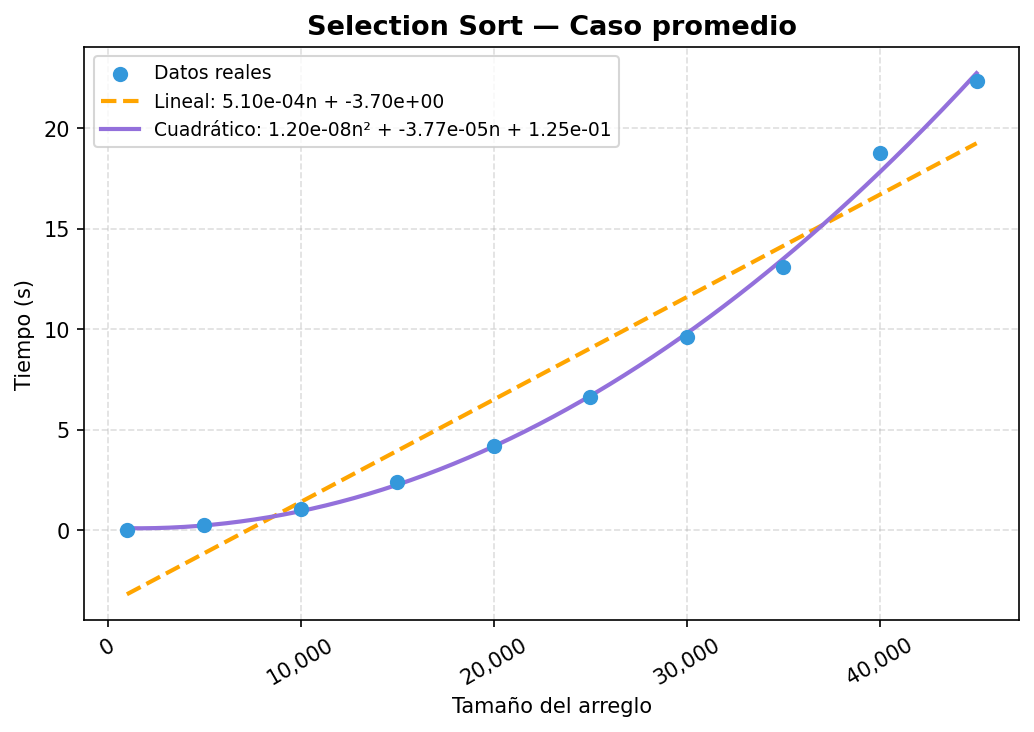
\includegraphics[width=0.6\textwidth]{graficas/selection_sort_aleatorio.png}
\caption{Ajuste por mínimos cuadrados para Selection Sort con arreglo aleatorio}
\label{fig:selection_average_fit}
\end{figure}



\newpage
\section{Merge Sort}
Una característica importante de Merge Sort es que su comportamiento no depende del orden inicial de los datos. Independientemente de si el arreglo está ordenado, invertido o aleatorio, el número de operaciones realizadas es aproximadamente el mismo.

\subsection{Implementación}
El código utilizado para implementar Merge Sort en Python es el siguiente:

\begin{lstlisting}
import math

def merge(arrOne, arrTwo):
    arrThree = []

    while arrOne and arrTwo:
        if arrOne[0] > arrTwo[0]:
            arrThree.append(arrTwo.pop(0)) 
        else:
            arrThree.append(arrOne.pop(0))

    while arrOne:
        arrThree.append(arrOne.pop(0))
    while arrTwo:
        arrThree.append(arrTwo.pop(0))

    return arrThree

def merge_sort(arr):
    if len(arr) <= 1:
        return arr
    
    mid = len(arr) // 2 
    arrOne = arr[:mid]
    arrTwo = arr[mid:]

    arrOne = merge_sort(arrOne)
    arrTwo = merge_sort(arrTwo)

    return merge(arrOne, arrTwo)
\end{lstlisting}


\newpage
\subsection{Resultados}
La tabla muestra los tiempos de ejecución obtenidos para los diferentes tamaños de arreglo y tipos de orden inicial.

\begin{table}[H]
\centering
\begin{tabular}{|l|c|r|}
\hline
Orden & Tamaño & Tiempo (s) \\
\hline
creciente & 1000 & 0.000697 \\
creciente & 5000 & 0.004626 \\
creciente & 10000 & 0.009434 \\
creciente & 15000 & 0.016547 \\
creciente & 20000 & 0.025854 \\
creciente & 25000 & 0.036803 \\
creciente & 30000 & 0.049358 \\
creciente & 35000 & 0.063865 \\
creciente & 40000 & 0.080087 \\
creciente & 45000 & 0.097537 \\
\hline
decreciente & 1000 & 0.000567 \\
decreciente & 5000 & 0.003788 \\
decreciente & 10000 & 0.009781 \\
decreciente & 15000 & 0.017211 \\
decreciente & 20000 & 0.026472 \\
decreciente & 25000 & 0.037388 \\
decreciente & 30000 & 0.050020 \\
decreciente & 35000 & 0.064202 \\
decreciente & 40000 & 0.080696 \\
decreciente & 45000 & 0.098243 \\
\hline
aleatorio & 1000 & 0.000666 \\
aleatorio & 5000 & 0.004499 \\
aleatorio & 10000 & 0.011232 \\
aleatorio & 15000 & 0.019709 \\
aleatorio & 20000 & 0.030211 \\
aleatorio & 25000 & 0.042028 \\
aleatorio & 30000 & 0.056170 \\
aleatorio & 35000 & 0.072857 \\
aleatorio & 40000 & 0.090833 \\
aleatorio & 45000 & 0.108540 \\
\hline
\end{tabular}
\caption{Tiempos de ejecución de Merge Sort}
\label{tab:merge_results}
\end{table}


\newpage
\subsection{Gráfica de resultados}
La figura muestra la relación entre el tamaño del arreglo y el tiempo de ejecución del algoritmo para los diferentes tipos de orden inicial.

\begin{figure}[H]
\centering
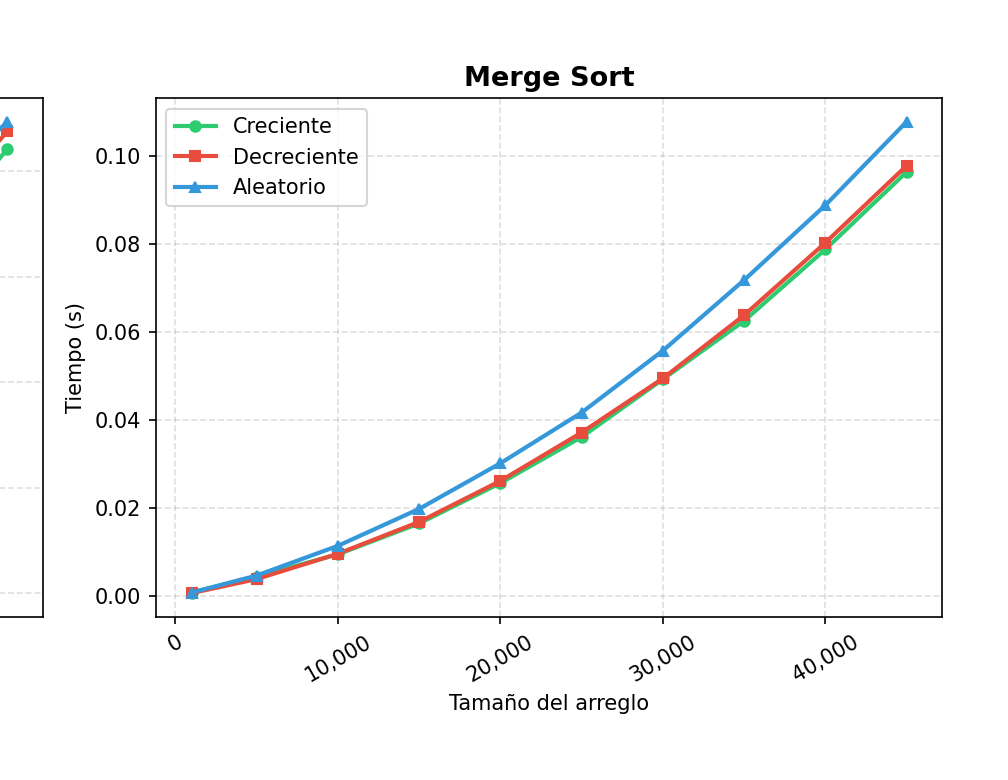
\includegraphics[width=0.6\textwidth]{graficas/merge_sort.png}
\caption{Tiempo de ejecución de Merge Sort}
\label{fig:merge_graph}
\end{figure}



\section{Jerarquía de crecimiento}
\begin{figure}[H]
\centering
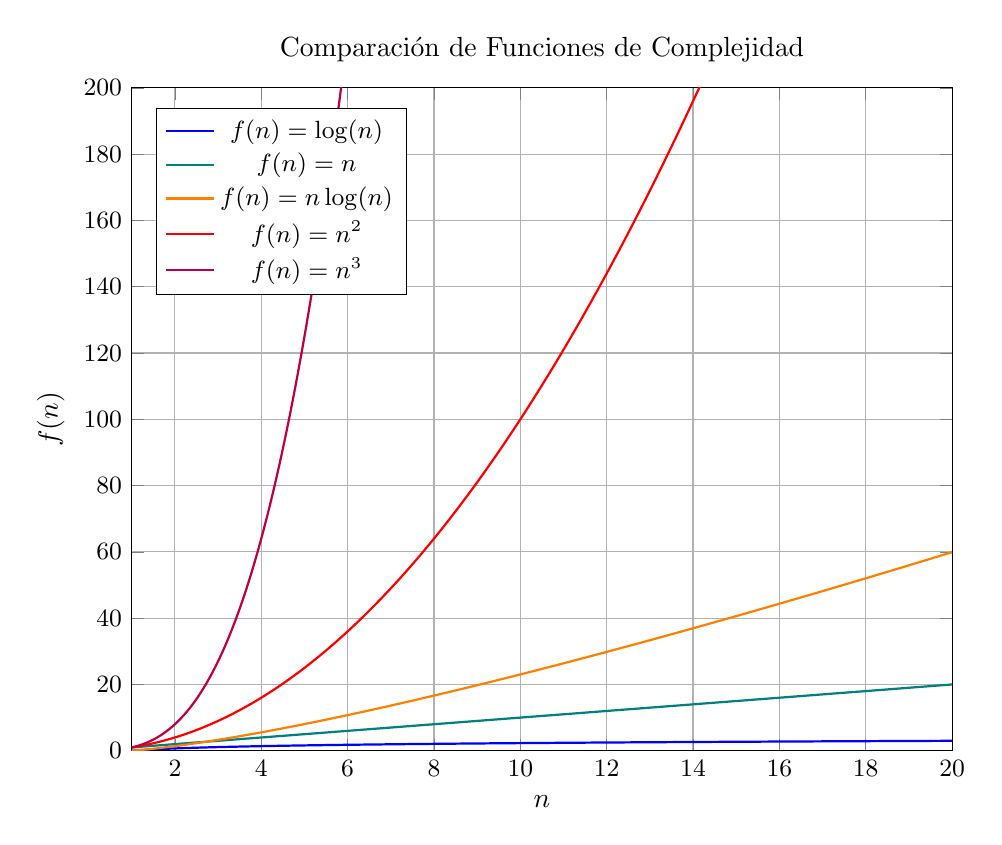
\begin{tikzpicture}
\begin{axis}[
    width=12cm, height=10cm,
    xmin=1, xmax=20,
    ymin=0, ymax=200,
    xlabel={$n$},
    ylabel={$f(n)$},
    title={Comparación de Funciones de Complejidad},
    legend pos=north west,
    legend style={font=\small},
    grid=both,
    grid style={line width=0.2pt, draw=gray!30},
    major grid style={line width=0.4pt, draw=gray!60},
    tick label style={font=\small},
    samples=200,
    smooth,
]

\addplot[blue,        thick, domain=1:20] {ln(x)};
\addplot[teal,        thick, domain=1:20] {x};
\addplot[orange,      thick, domain=1:20] {x * ln(x)};
\addplot[red,         thick, domain=1:20] {x^2};
\addplot[purple,      thick, domain=1:20] {x^3};

\legend{
    $f(n) = \log(n)$,
    $f(n) = n$,
    $f(n) = n\log(n)$,
    $f(n) = n^2$,
    $f(n) = n^3$
}

\end{axis}
\end{tikzpicture}
\end{figure}
\end{document}
